\documentclass{standalone}

\usepackage{tikz}
\usepackage{circuitikz}

\tikzset{block/.style = {draw, fill=white, very thick, rectangle, minimum height=1cm, minimum width=2cm},
         lblock/.style={draw,fill=white,very thick, rectangle, minimum height=3cm, minimum width=1cm},
         sum/.style= {draw, fill=white, very thick, circle, node distance=0.5cm}}

         
\begin{document}
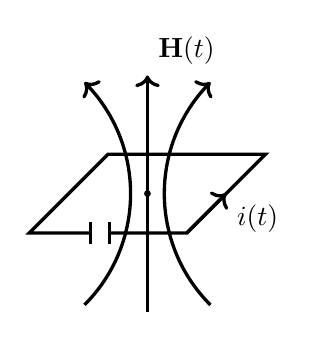
\begin{tikzpicture}[scale=2]
    \draw[|-|, very thick](-0.25,-0.25)--(0.25,-0.25)--(0.75,0.25)--(-0.25,0.25)--(-0.75,-0.25)--(-0.35,-0.25);
    \draw[->, very thick](0.25,-0.25)--(0.5,0)node[below right]{$i(t)$};

    \draw[->, very thick](0,-0.75)--(0,0.75)node[above right]{$\mathbf{H}(t)$};
    \filldraw[black](0,0)circle(0.5pt);

    \draw[->, very thick](-0.4,-0.707)arc(-45:45:1);
    \draw[->, very thick](0.4,-0.707)arc(225:135:1);
\end{tikzpicture}
\end{document}